\documentclass{article}
\usepackage[utf8]{inputenc}
\usepackage[euler]{textgreek}
\usepackage{amsmath}
\usepackage{amsfonts}
\usepackage{tabularx}
\usepackage{layout}
\usepackage{geometry}
\usepackage{calc}
\usepackage{siunitx}
\usepackage{graphicx}
\usepackage{listings}
\usepackage{xcolor}
\usepackage{longtable}
\usepackage{soul}
\usepackage{calligra}
\usepackage{mathtools}
\usepackage{float}
\usepackage{subfig}
\usepackage{subcaption}
\usepackage{mdframed}
\usepackage{gensymb}


\setlength{\hoffset}{0in}
\setlength{\voffset}{0in}
\setlength{\oddsidemargin}{0px}
\setlength{\headheight}{0em}
\setlength{\headsep}{0em}
\setlength{\marginparwidth}{0em}
\setlength{\marginparsep}{0em}
\setlength{\textheight}{\paperheight - 2in}
\setlength{\textwidth}{\paperwidth - 2in}

\setlength{\parindent}{1.5em}
\setlength{\parskip}{0.5em}
\setlength{\tabcolsep}{0.2em}

\newcolumntype{C}{>{\centering\arraybackslash}X}

\newcommand{\hlc}[2][yellow]{{%
    \colorlet{foo}{#1}%
    \sethlcolor{foo}\hl{#2}}%
}

\newcommand*{\ZZ}{%
  \textsf{Z\kern-1ex Z}%
}

\newmdenv[leftline=false,rightline=false,topline=false,skipabove=5mm,skipbelow=0,leftmargin=0,innertopmargin=0mm,innerbottommargin=0.5mm,innerleftmargin=0]{largeUnderline}
\newcommand{\expart}[1]
{
    \begin{largeUnderline}#1\end{largeUnderline}\par
}

% Pour les dx
\newcommand*\dif{\mathop{}\!\mathrm{d}}

% Pour faire dx/dt
\newcommand{\deriv}[1]{
    \frac{\dif #1}{\dif t}
}

\newcommand{\derivn}[2]{
    \frac{\dif^{#2} #1}{\dif t^{#2}}
}

% *10^x
\newcommand{\e}[1]{
    \times 10^{#1}
}

% Inclure du texte dans dans des environnements de maths avec des marges pas trop dégelasses
\newcommand{\txt}[1]{
    \;\;\text{#1}\;\;
}

% Unités
\newcommand{\un}[1]{
    \,\text{#1}
}

% Puissances pour unités, attention pour les lettres grecques il faut utiliser \text[letter] au lieu de \[letter]
\newcommand{\p}[1]{
    \!$^{#1}$\!\!\!
}

% Puissance -1
\newcommand{\pmo}{
    \!\!\!$^{-1}$\!\!\!
}

\newcommand{\apriori}{{\it a priori} }

\newcommand{\ub}[1]{\underline{#1}}

% Valeur absolue
\DeclarePairedDelimiter\abs{\lvert}{\rvert}

\begin{document}

Chollet Arthur

\begin{center}
    \Huge
    \normalfont\calligra Compte-rendu capacité numérique: effet du filtrage
\end{center}

\expart{1. FFT}

Pour avoir la magnitude du signal on prend le module $\left(\sqrt{Re^2 + Im^2}\right)$ de chaque éléments dans la liste du resultat de la fft. Ainsi pour avoir l'amplitude on a juste a multiplié par 2 et diviser par le nombre d'échantillonage

Pour obtenir la fréquence il suffit de diviser par la durée d'échantillonage notre position actuelle dans liste du résultat de la fft.

Pour déterminer la phase, on prend l'argument $\left(\arctan\left(\frac{Im}{Re}\right)\right)$ de chaque éléments dans la liste du resultat de la fft 

La sortie est continue et pleine d'imperfections, ainsi on la traite en programmant un algorithme de détection de 'piques' pour ensuite uniquement tracé ces 'piques'

\begin{figure}[H]
  \centering
  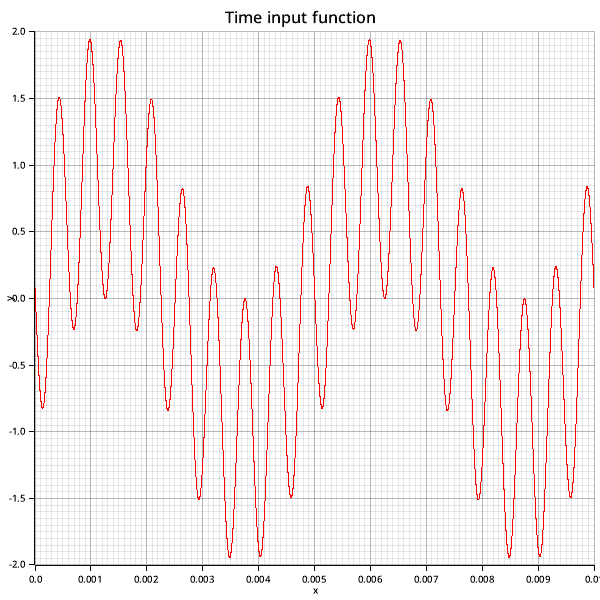
\includegraphics[height=15em]{images/custom/fft_test/sin_time_input.png}
  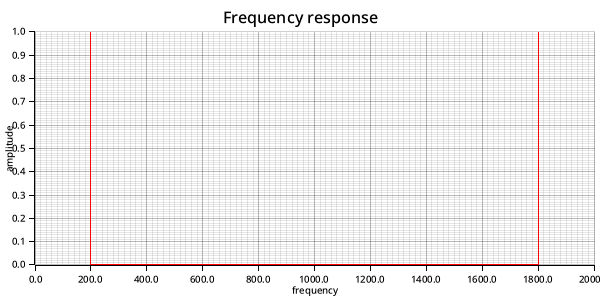
\includegraphics[height=13em]{images/custom/fft_test/sin_fft_result.png}
  \caption{Teste de la fonction fft avec une signal composé de 2 sinus d'amplitude 1 et de fréquence 200Hz et 1800Hz}
\end{figure}

En codant une fonction permettant de générer un signal créneau et un signal triangulaire tel que:

\begin{align*}
  &Creneau(t) = \begin{cases}
    A \text{ si } 0<t<\frac{T}{2}\\
    B \text{ si } \frac{T}{2}<t<T
  \end{cases}\\
  &Triangle(t) = \begin{cases}
    \frac{2(B-A)}{T}t+A \text{ si } 0<t<\frac{T}{2}\\
    \frac{2(A-B)}{T}t+2B-A \text{ si } \frac{T}{2}<t<T
  \end{cases}
\end{align*}

Nous obtenons les spectres suivants:

\begin{figure}[H]
  \centering
  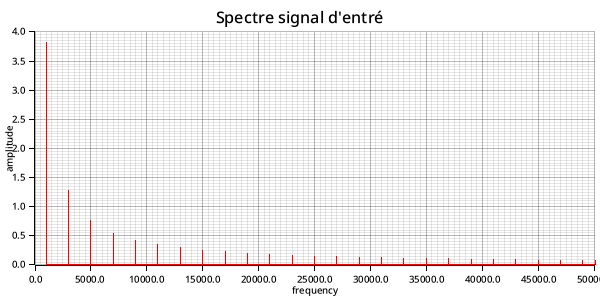
\includegraphics[height=15em]{images/creneau/fft_in.png}
  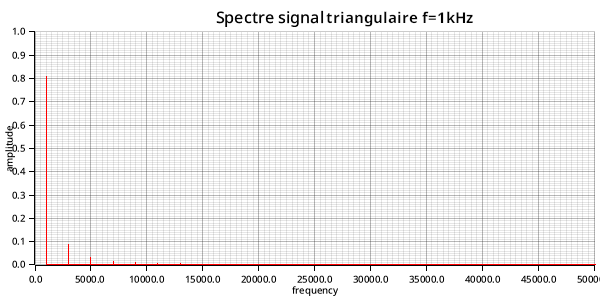
\includegraphics[height=15em]{images/triangulaire/fft_in.png}
  \caption{Spectre d'un signal créneau et d'un signal triangulaire de fréquence 1kHz}
\end{figure}

\expart{2.1 Simulation de l'effet de filtres sur un signal quelconque}

On code à la main et une par une les fonctions de gains et de phases pour les 4 types de filtres utilisé ici: Passe bas/haut du 1er ordre, passe bande, coupe bande 

Remarque: des expérimentations avec les filtre passe bas/haut du 2nd ordre ont été réalisé mais afin de réduire la taille de ce compte-rendu j'ai décidé de ne pas les incorporer.

Pour chaque fréquence détectée dans la transformée de Fourier du signal d'entrée, on multiplie son amplitude par le gain correspondant du filtre à cette fréquence, ce qui détermine l'amplitude de sortie à cette fréquence. Ensuite, on additionne à la phase d'entrée à cette fréquence la valeur correspondante de la phase du filtre, aboutissant ainsi à la phase de sortie à cette fréquence.

\begin{figure}[H]
  \begin{minipage}{0.6\textwidth}
      \centering
      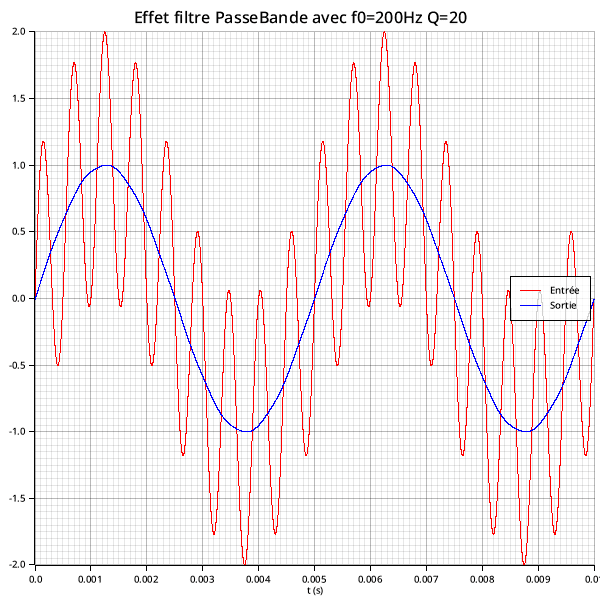
\includegraphics[width=25em]{images/custom/filtrage_test/signals.png}
  \end{minipage}
  \begin{minipage}{0.3\textwidth}
      \centering
      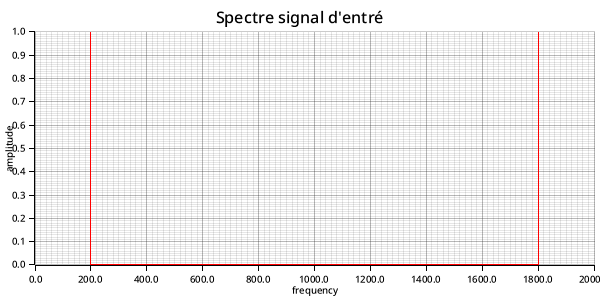
\includegraphics[width=16em]{images/custom/filtrage_test/fft_in.png}
      \vfill
      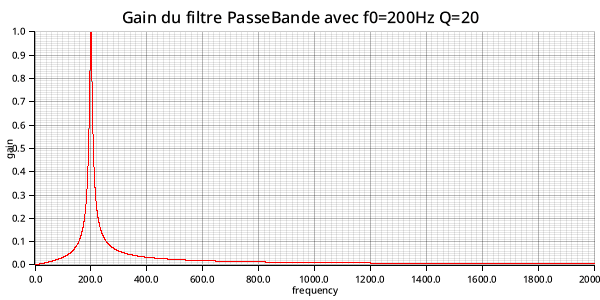
\includegraphics[width=16em]{images/custom/filtrage_test/gain.png}
      \vfill
      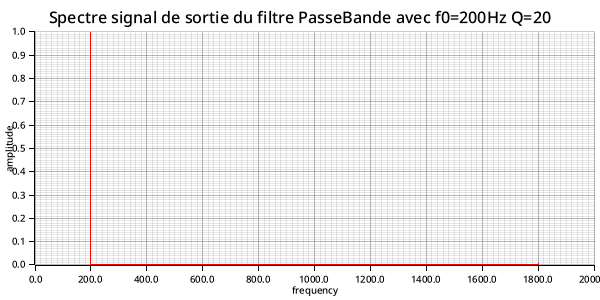
\includegraphics[width=16em]{images/custom/filtrage_test/fft_out.png}
  \end{minipage}
  \caption{Effet d'un filtre passe bande sur un signal composé de 2 fréquence, dont une coupé}
\end{figure}

\expart{2.2 Simulation de l'effet de filtres sur un signal créneau}

On prendra pour toute la suite un signal créneau de fréquence $f=1$kHz de valeur moyenne 1V et d'amplitude 3V

Voici le spectre du créneau d'entrée:

\begin{figure}[H]
  \centering
  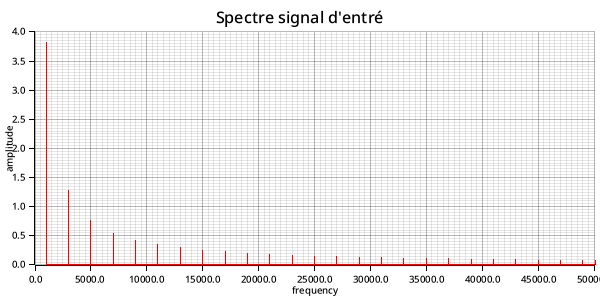
\includegraphics[height=15em]{images/creneau/fft_in.png}
  \caption{Spectre du signal créneau en entré de fréquence 1kHz}
\end{figure}

\expart{2.2.1 Filtrage par filtre passe bas}

\begin{figure}[H]
  \begin{minipage}{0.6\textwidth}
      \centering
      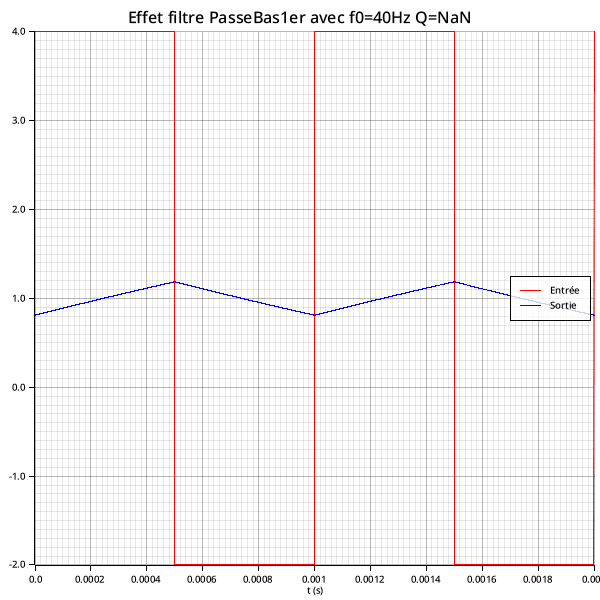
\includegraphics[width=25em]{images/creneau/bas/0.04/signals.png}
  \end{minipage}
  \begin{minipage}{0.3\textwidth}
      \centering
      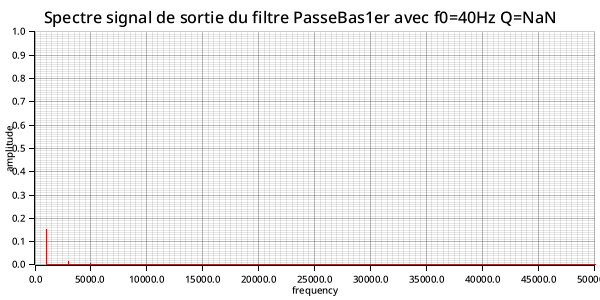
\includegraphics[width=16em]{images/creneau/bas/0.04/fft_out.png}
      \vfill
      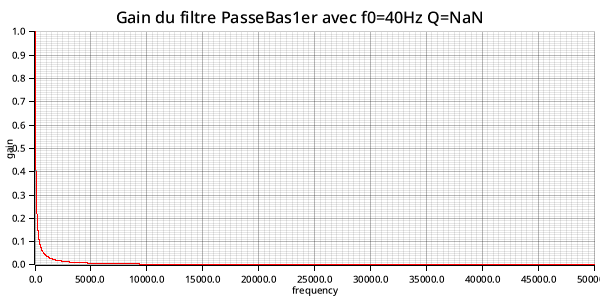
\includegraphics[width=16em]{images/creneau/bas/0.04/gain.png}
      \vfill
      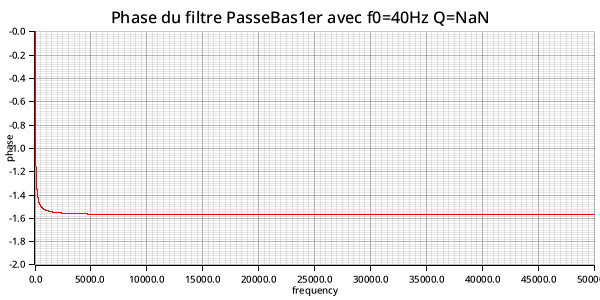
\includegraphics[width=16em]{images/creneau/bas/0.04/phase.png}
  \end{minipage}
  \caption{Effet passe bas pour $f_0=0.04f$}
\end{figure}

\begin{figure}[H]
  \begin{minipage}{0.6\textwidth}
      \centering
      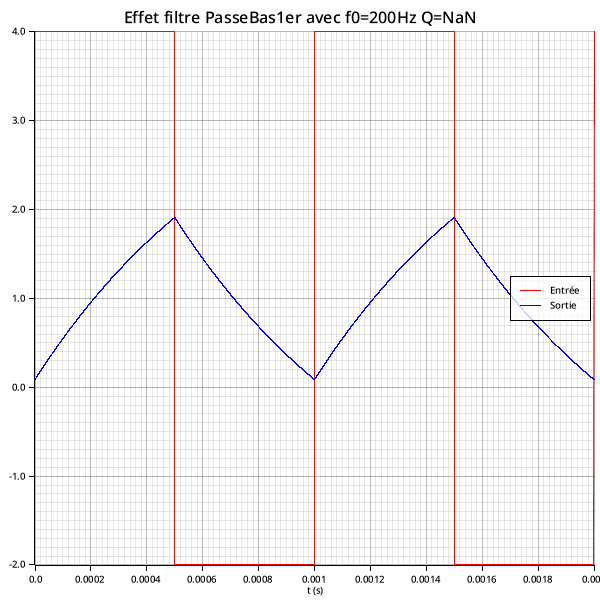
\includegraphics[width=25em]{images/creneau/bas/0.2/signals.png}
  \end{minipage}
  \begin{minipage}{0.3\textwidth}
      \centering
      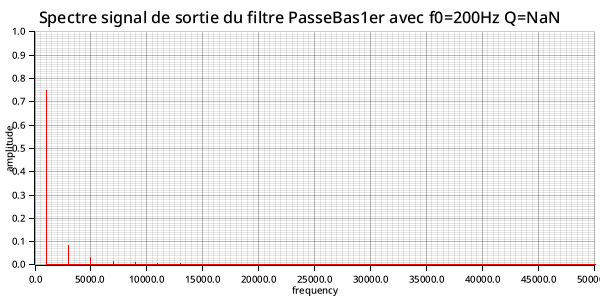
\includegraphics[width=16em]{images/creneau/bas/0.2/fft_out.png}
      \vfill
      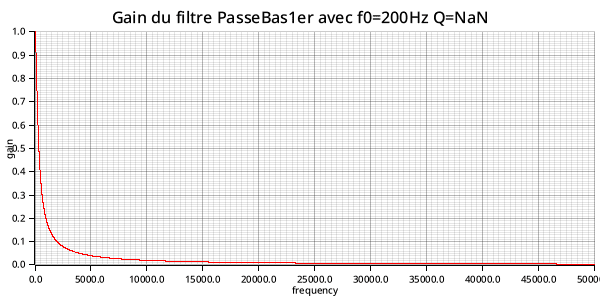
\includegraphics[width=16em]{images/creneau/bas/0.2/gain.png}
      \vfill
      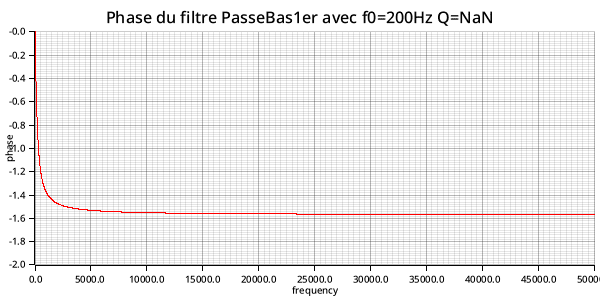
\includegraphics[width=16em]{images/creneau/bas/0.2/phase.png}
  \end{minipage}
  \caption{Effet passe bas pour $f_0=0.2f$}
\end{figure}

\begin{figure}[H]
  \begin{minipage}{0.6\textwidth}
      \centering
      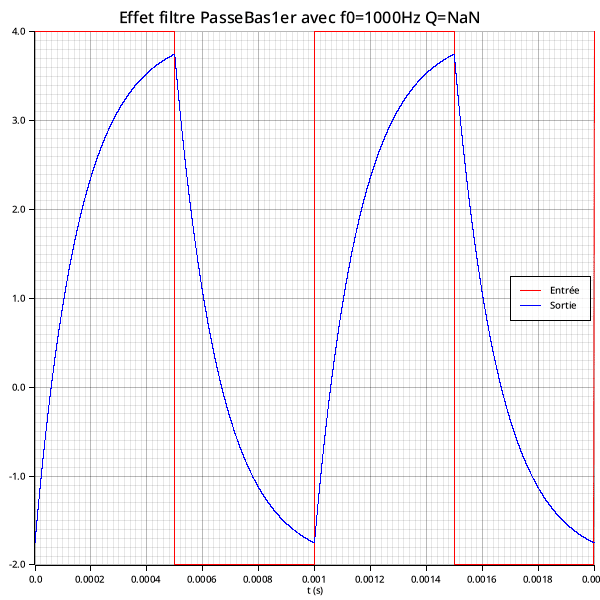
\includegraphics[width=25em]{images/creneau/bas/1/signals.png}
  \end{minipage}
  \begin{minipage}{0.3\textwidth}
      \centering
      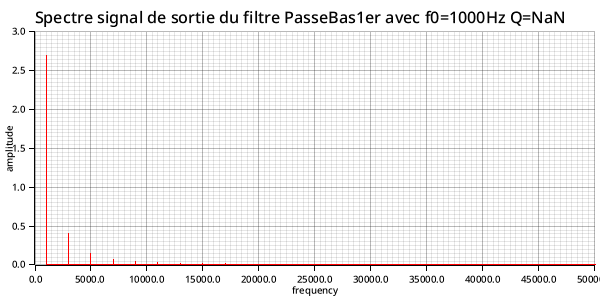
\includegraphics[width=16em]{images/creneau/bas/1/fft_out.png}
      \vfill
      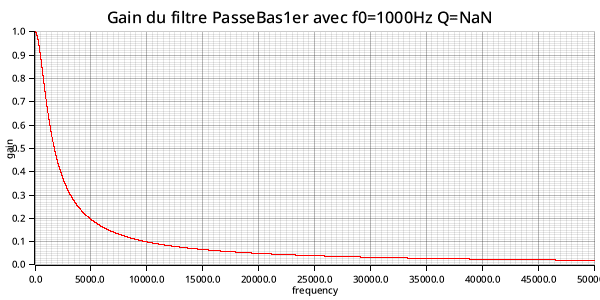
\includegraphics[width=16em]{images/creneau/bas/1/gain.png}
      \vfill
      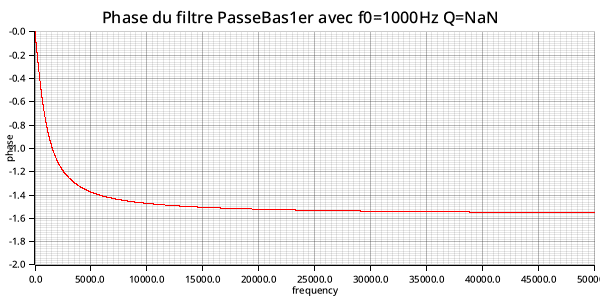
\includegraphics[width=16em]{images/creneau/bas/1/phase.png}
  \end{minipage}
  \caption{Effet passe bas pour $f_0=f$}
\end{figure}

\begin{figure}[H]
  \begin{minipage}{0.6\textwidth}
      \centering
      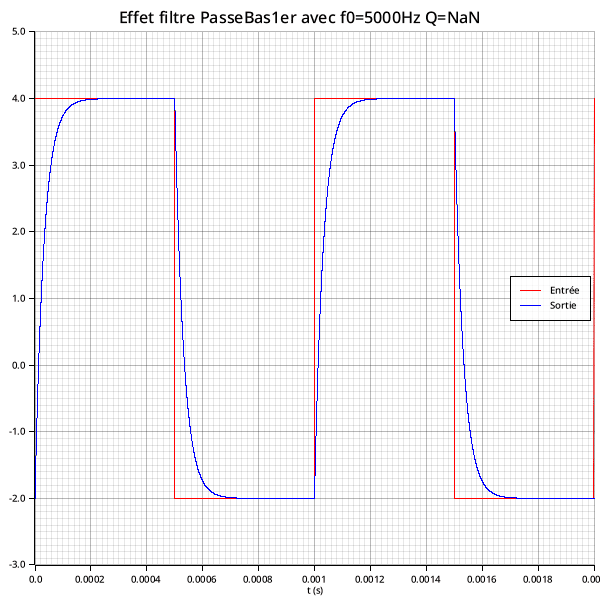
\includegraphics[width=25em]{images/creneau/bas/5/signals.png}
  \end{minipage}
  \begin{minipage}{0.3\textwidth}
      \centering
      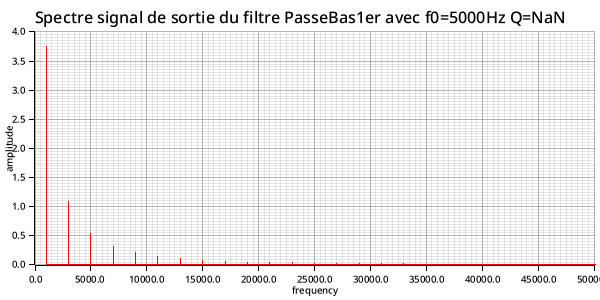
\includegraphics[width=16em]{images/creneau/bas/5/fft_out.png}
      \vfill
      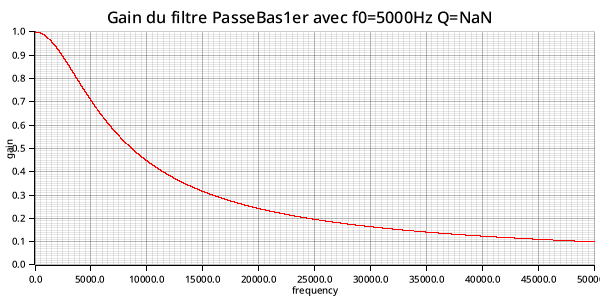
\includegraphics[width=16em]{images/creneau/bas/5/gain.png}
      \vfill
      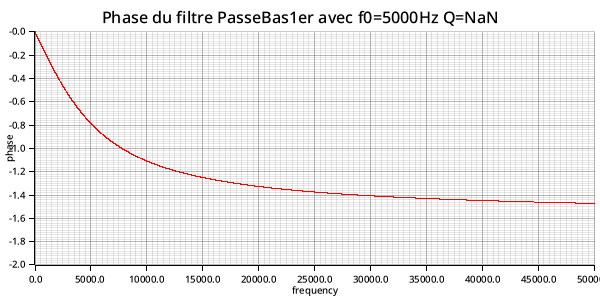
\includegraphics[width=16em]{images/creneau/bas/5/phase.png}
  \end{minipage}
  \caption{Effet passe bas pour $f_0=5f$}
\end{figure}

\begin{figure}[H]
  \begin{minipage}{0.6\textwidth}
      \centering
      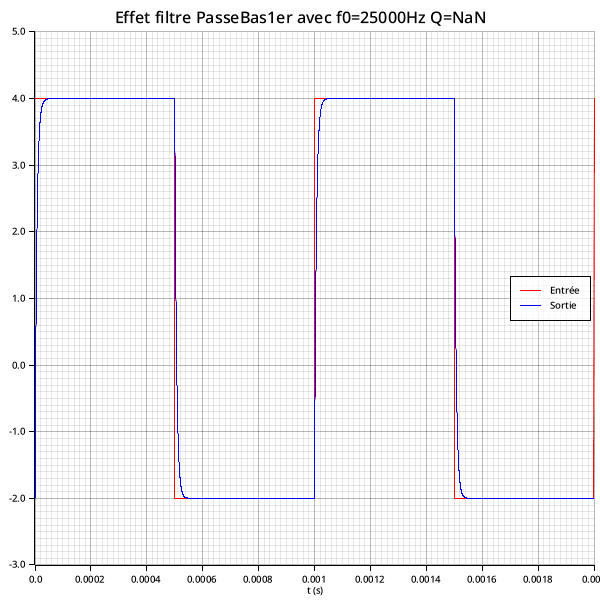
\includegraphics[width=25em]{images/creneau/bas/25/signals.png}
  \end{minipage}
  \begin{minipage}{0.3\textwidth}
      \centering
      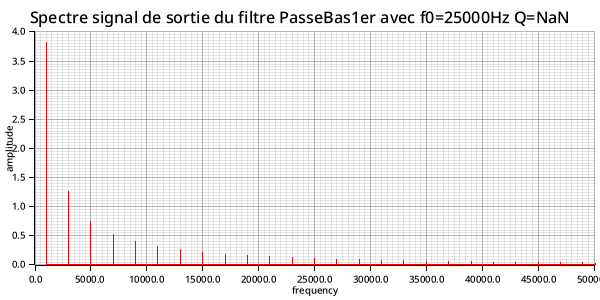
\includegraphics[width=16em]{images/creneau/bas/25/fft_out.png}
      \vfill
      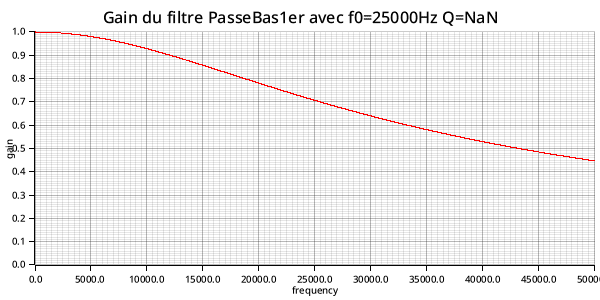
\includegraphics[width=16em]{images/creneau/bas/25/gain.png}
      \vfill
      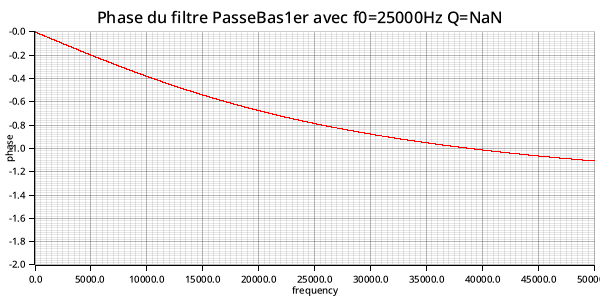
\includegraphics[width=16em]{images/creneau/bas/25/phase.png}
  \end{minipage}
  \caption{Effet passe bas pour $f_0=25f$}
\end{figure}

\expart{2.2.2 Filtrage par filtre passe haut}

\begin{figure}[H]
  \begin{minipage}{0.6\textwidth}
      \centering
      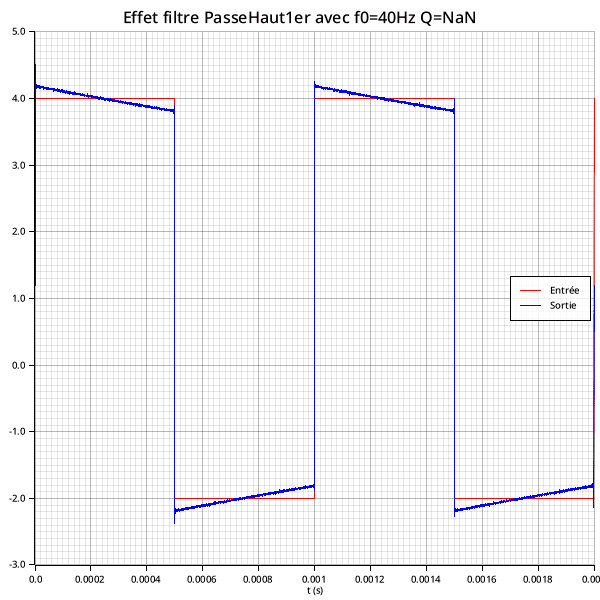
\includegraphics[width=25em]{images/creneau/haut/0.04/signals.png}
  \end{minipage}
  \begin{minipage}{0.3\textwidth}
      \centering
      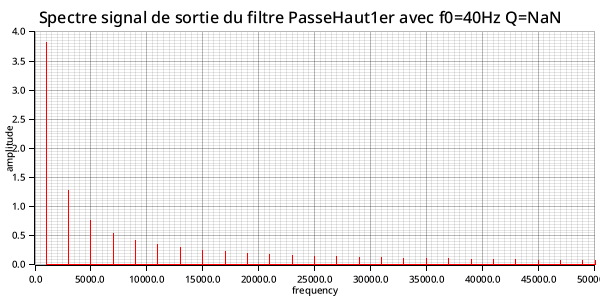
\includegraphics[width=16em]{images/creneau/haut/0.04/fft_out.png}
      \vfill
      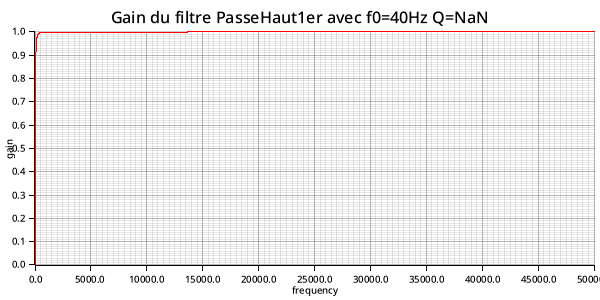
\includegraphics[width=16em]{images/creneau/haut/0.04/gain.png}
      \vfill
      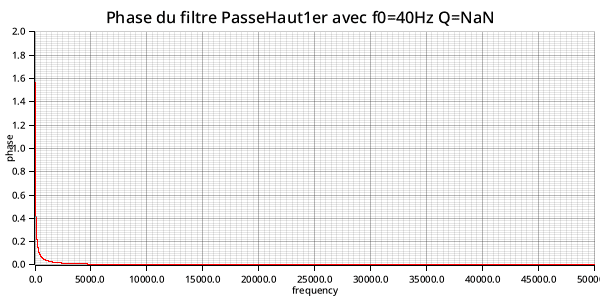
\includegraphics[width=16em]{images/creneau/haut/0.04/phase.png}
  \end{minipage}
  \caption{Effet passe haut pour $f_0=0.04f$}
\end{figure}

\begin{figure}[H]
  \begin{minipage}{0.6\textwidth}
      \centering
      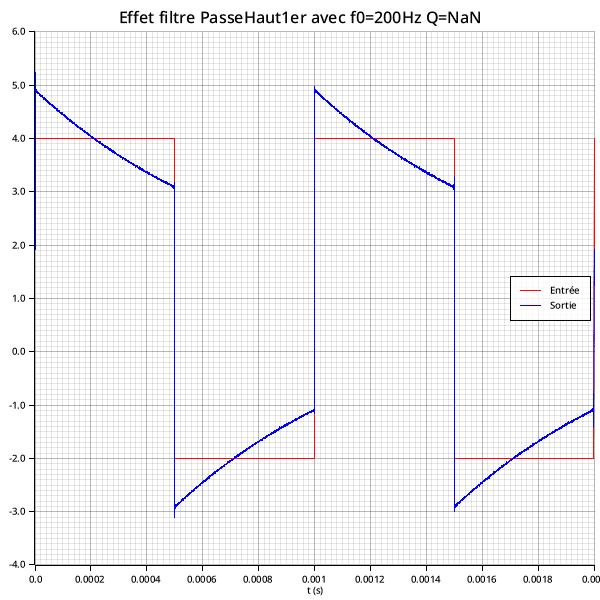
\includegraphics[width=25em]{images/creneau/haut/0.2/signals.png}
  \end{minipage}
  \begin{minipage}{0.3\textwidth}
      \centering
      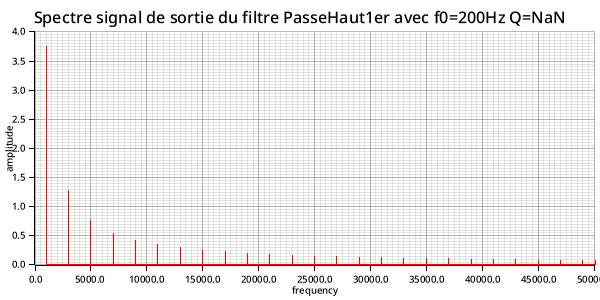
\includegraphics[width=16em]{images/creneau/haut/0.2/fft_out.png}
      \vfill
      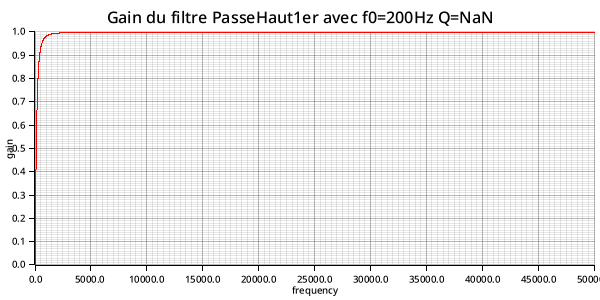
\includegraphics[width=16em]{images/creneau/haut/0.2/gain.png}
      \vfill
      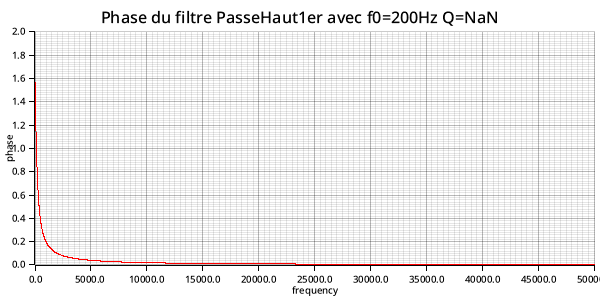
\includegraphics[width=16em]{images/creneau/haut/0.2/phase.png}
  \end{minipage}
  \caption{Effet passe haut pour $f_0=0.2f$}
\end{figure}

\begin{figure}[H]
  \begin{minipage}{0.6\textwidth}
      \centering
      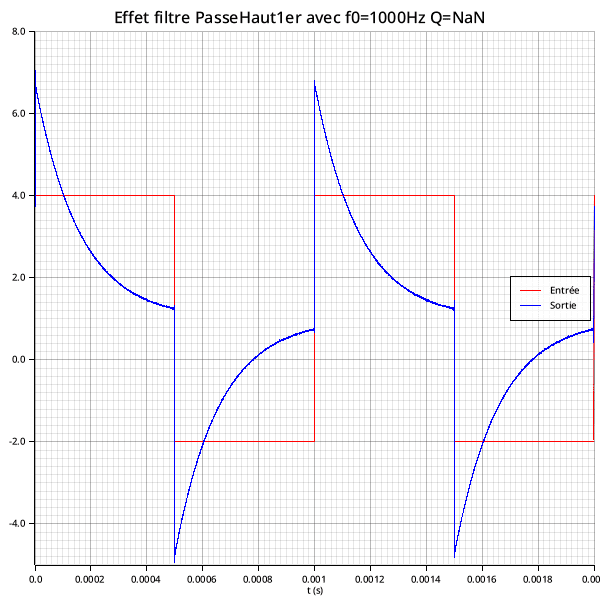
\includegraphics[width=25em]{images/creneau/haut/1/signals.png}
  \end{minipage}
  \begin{minipage}{0.3\textwidth}
      \centering
      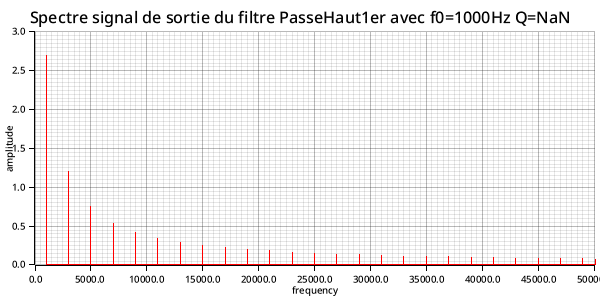
\includegraphics[width=16em]{images/creneau/haut/1/fft_out.png}
      \vfill
      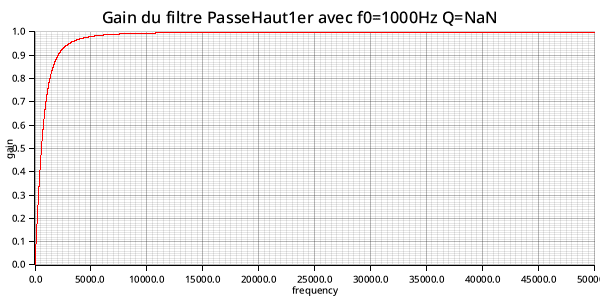
\includegraphics[width=16em]{images/creneau/haut/1/gain.png}
      \vfill
      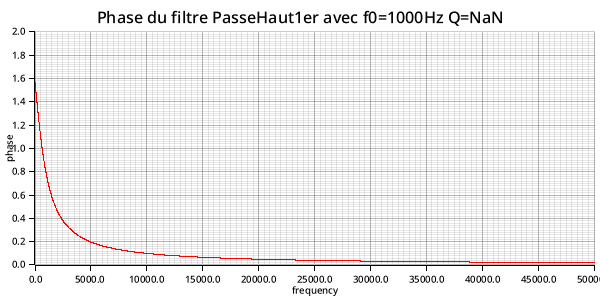
\includegraphics[width=16em]{images/creneau/haut/1/phase.png}
  \end{minipage}
  \caption{Effet passe haut pour $f_0=f$}
\end{figure}

\begin{figure}[H]
  \begin{minipage}{0.6\textwidth}
      \centering
      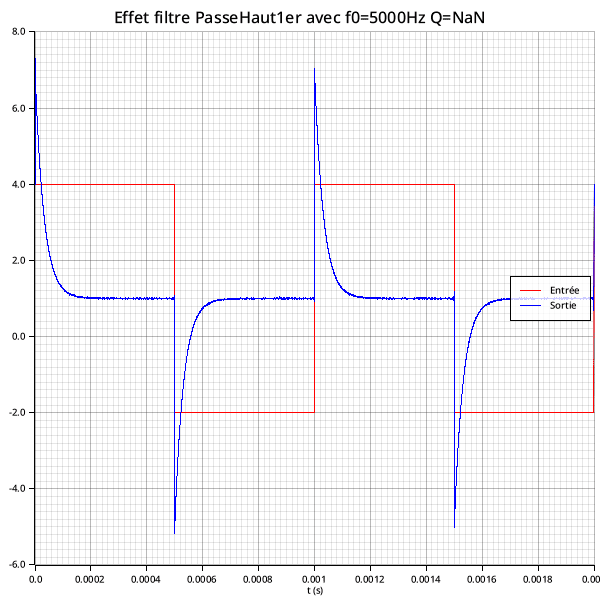
\includegraphics[width=25em]{images/creneau/haut/5/signals.png}
  \end{minipage}
  \begin{minipage}{0.3\textwidth}
      \centering
      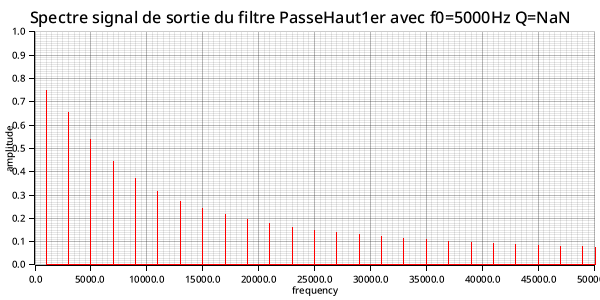
\includegraphics[width=16em]{images/creneau/haut/5/fft_out.png}
      \vfill
      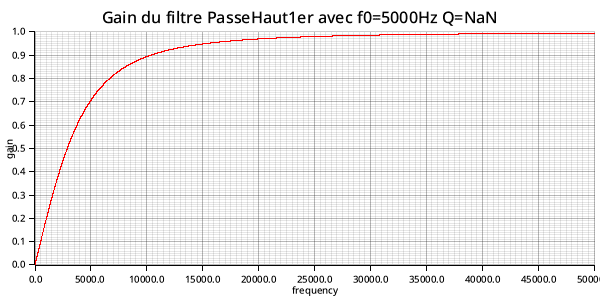
\includegraphics[width=16em]{images/creneau/haut/5/gain.png}
      \vfill
      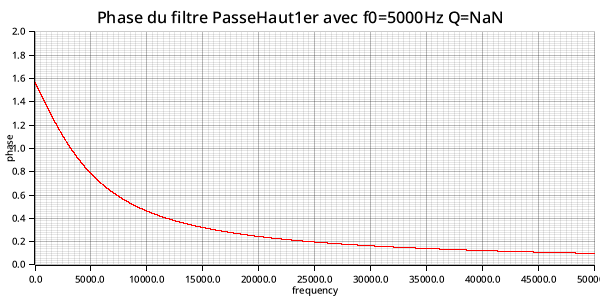
\includegraphics[width=16em]{images/creneau/haut/5/phase.png}
  \end{minipage}
  \caption{Effet passe haut pour $f_0=5f$}
\end{figure}

\begin{figure}[H]
  \begin{minipage}{0.6\textwidth}
      \centering
      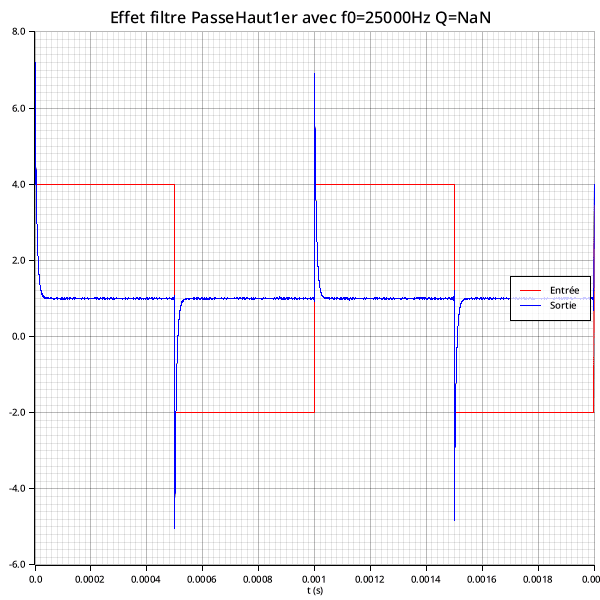
\includegraphics[width=25em]{images/creneau/haut/25/signals.png}
  \end{minipage}
  \begin{minipage}{0.3\textwidth}
      \centering
      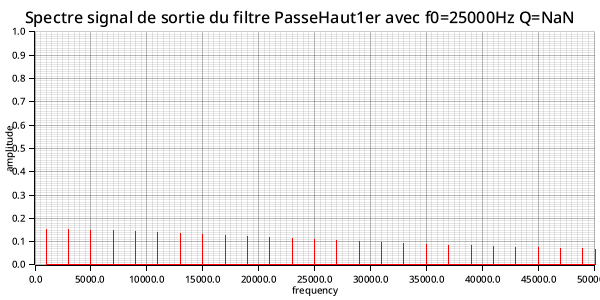
\includegraphics[width=16em]{images/creneau/haut/25/fft_out.png}
      \vfill
      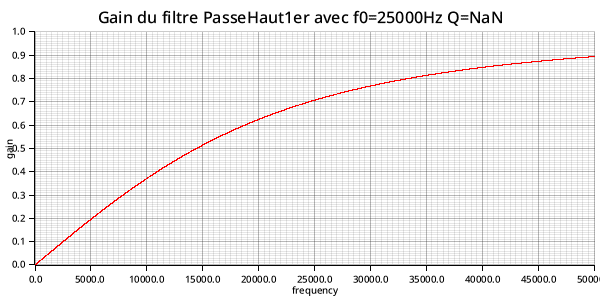
\includegraphics[width=16em]{images/creneau/haut/25/gain.png}
      \vfill
      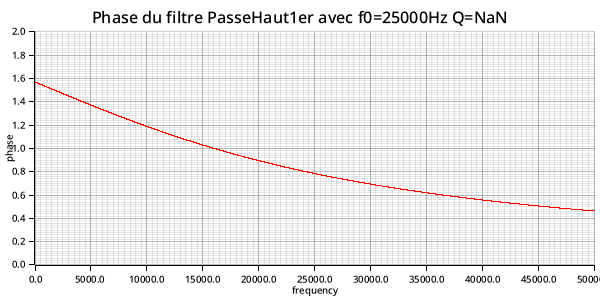
\includegraphics[width=16em]{images/creneau/haut/25/phase.png}
  \end{minipage}
  \caption{Effet passe haut pour $f_0=25f$}
\end{figure}

\pagebreak

\expart{2.2.3 Filtrage par filtre passe bande}

\begin{figure}[H]
  \begin{minipage}{0.6\textwidth}
      \centering
      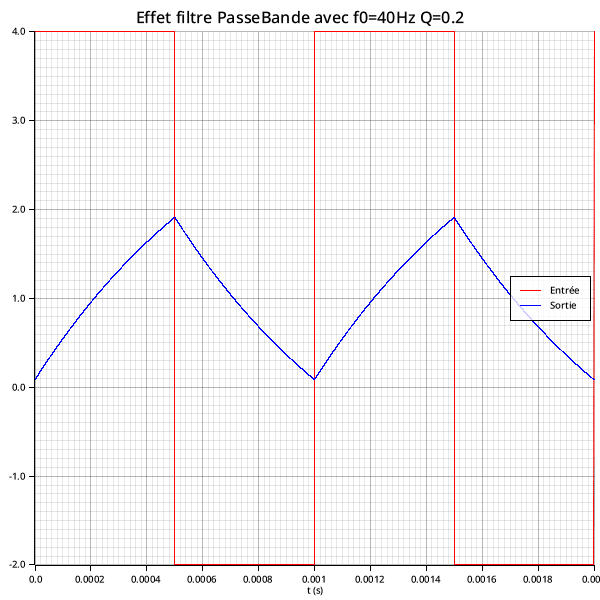
\includegraphics[width=25em]{images/creneau/bande/q=0.2/0.04/signals.png}
  \end{minipage}
  \begin{minipage}{0.3\textwidth}
      \centering
      \includegraphics[width=16em]{images/creneau/bande/q=0.2/0.04/fft_out.png}
      \vfill
      \includegraphics[width=16em]{images/creneau/bande/q=0.2/0.04/gain.png}
      \vfill
      \includegraphics[width=16em]{images/creneau/bande/q=0.2/0.04/phase.png}
  \end{minipage}
  \caption{Effet passe bande pour $f_0=0.04f$ et $Q=0.2$}
\end{figure}

\begin{figure}[H]
  \begin{minipage}{0.6\textwidth}
      \centering
      \includegraphics[width=25em]{images/creneau/bande/q=0.2/0.2/signals.png}
  \end{minipage}
  \begin{minipage}{0.3\textwidth}
      \centering
      \includegraphics[width=16em]{images/creneau/bande/q=0.2/0.2/fft_out.png}
      \vfill
      \includegraphics[width=16em]{images/creneau/bande/q=0.2/0.2/gain.png}
      \vfill
      \includegraphics[width=16em]{images/creneau/bande/q=0.2/0.2/phase.png}
  \end{minipage}
  \caption{Effet passe bande pour $f_0=0.2f$ et $Q=0.2$}
\end{figure}

\begin{figure}[H]
  \begin{minipage}{0.6\textwidth}
      \centering
      \includegraphics[width=25em]{images/creneau/bande/q=0.2/1/signals.png}
  \end{minipage}
  \begin{minipage}{0.3\textwidth}
      \centering
      \includegraphics[width=16em]{images/creneau/bande/q=0.2/1/fft_out.png}
      \vfill
      \includegraphics[width=16em]{images/creneau/bande/q=0.2/1/gain.png}
      \vfill
      \includegraphics[width=16em]{images/creneau/bande/q=0.2/1/phase.png}
  \end{minipage}
  \caption{Effet passe bande pour $f_0=f$ et $Q=0.2$}
\end{figure}

\begin{figure}[H]
  \begin{minipage}{0.6\textwidth}
      \centering
      \includegraphics[width=25em]{images/creneau/bande/q=0.2/5/signals.png}
  \end{minipage}
  \begin{minipage}{0.3\textwidth}
      \centering
      \includegraphics[width=16em]{images/creneau/bande/q=0.2/5/fft_out.png}
      \vfill
      \includegraphics[width=16em]{images/creneau/bande/q=0.2/5/gain.png}
      \vfill
      \includegraphics[width=16em]{images/creneau/bande/q=0.2/5/phase.png}
  \end{minipage}
  \caption{Effet passe bande pour $f_0=5f$ et $Q=0.2$}
\end{figure}

\begin{figure}[H]
  \begin{minipage}{0.6\textwidth}
      \centering
      \includegraphics[width=25em]{images/creneau/bande/q=0.2/25/signals.png}
  \end{minipage}
  \begin{minipage}{0.3\textwidth}
      \centering
      \includegraphics[width=16em]{images/creneau/bande/q=0.2/25/fft_out.png}
      \vfill
      \includegraphics[width=16em]{images/creneau/bande/q=0.2/25/gain.png}
      \vfill
      \includegraphics[width=16em]{images/creneau/bande/q=0.2/25/phase.png}
  \end{minipage}
  \caption{Effet passe bande pour $f_0=25f$ et $Q=0.2$}
\end{figure}

\begin{figure}[H]
  \begin{minipage}{0.6\textwidth}
      \centering
      \includegraphics[width=25em]{images/creneau/bande/q=20/0.04/signals.png}
  \end{minipage}
  \begin{minipage}{0.3\textwidth}
      \centering
      \includegraphics[width=16em]{images/creneau/bande/q=20/0.04/fft_out.png}
      \vfill
      \includegraphics[width=16em]{images/creneau/bande/q=20/0.04/gain.png}
      \vfill
      \includegraphics[width=16em]{images/creneau/bande/q=20/0.04/phase.png}
  \end{minipage}
  \caption{Effet passe bande pour $f_0=0.04f$ et $Q=20$}
\end{figure}

\begin{figure}[H]
  \begin{minipage}{0.6\textwidth}
      \centering
      \includegraphics[width=25em]{images/creneau/bande/q=20/0.2/signals.png}
  \end{minipage}
  \begin{minipage}{0.3\textwidth}
      \centering
      \includegraphics[width=16em]{images/creneau/bande/q=20/0.2/fft_out.png}
      \vfill
      \includegraphics[width=16em]{images/creneau/bande/q=20/0.2/gain.png}
      \vfill
      \includegraphics[width=16em]{images/creneau/bande/q=20/0.2/phase.png}
  \end{minipage}
  \caption{Effet passe bande pour $f_0=0.2f$ et $Q=20$}
\end{figure}

\begin{figure}[H]
  \begin{minipage}{0.6\textwidth}
      \centering
      \includegraphics[width=25em]{images/creneau/bande/q=20/1/signals.png}
  \end{minipage}
  \begin{minipage}{0.3\textwidth}
      \centering
      \includegraphics[width=16em]{images/creneau/bande/q=20/1/fft_out.png}
      \vfill
      \includegraphics[width=16em]{images/creneau/bande/q=20/1/gain.png}
      \vfill
      \includegraphics[width=16em]{images/creneau/bande/q=20/1/phase.png}
  \end{minipage}
  \caption{Effet passe bande pour $f_0=f$ et $Q=20$}
\end{figure}

\begin{figure}[H]
  \begin{minipage}{0.6\textwidth}
      \centering
      \includegraphics[width=25em]{images/creneau/bande/q=20/5/signals.png}
  \end{minipage}
  \begin{minipage}{0.3\textwidth}
      \centering
      \includegraphics[width=16em]{images/creneau/bande/q=20/5/fft_out.png}
      \vfill
      \includegraphics[width=16em]{images/creneau/bande/q=20/5/gain.png}
      \vfill
      \includegraphics[width=16em]{images/creneau/bande/q=20/5/phase.png}
  \end{minipage}
  \caption{Effet passe bande pour $f_0=5f$ et $Q=20$}
\end{figure}

\begin{figure}[H]
  \begin{minipage}{0.6\textwidth}
      \centering
      \includegraphics[width=25em]{images/creneau/bande/q=20/25/signals.png}
  \end{minipage}
  \begin{minipage}{0.3\textwidth}
      \centering
      \includegraphics[width=16em]{images/creneau/bande/q=20/25/fft_out.png}
      \vfill
      \includegraphics[width=16em]{images/creneau/bande/q=20/25/gain.png}
      \vfill
      \includegraphics[width=16em]{images/creneau/bande/q=20/25/phase.png}
  \end{minipage}
  \caption{Effet passe bande pour $f_0=25f$ et $Q=20$}
\end{figure}

\pagebreak

\expart{2.2.4 Filtrage par filtre coupe bande}

\begin{figure}[H]
  \begin{minipage}{0.6\textwidth}
      \centering
      \includegraphics[width=25em]{images/creneau/rejecteur/q=0.2/0.04/signals.png}
  \end{minipage}
  \begin{minipage}{0.3\textwidth}
      \centering
      \includegraphics[width=16em]{images/creneau/rejecteur/q=0.2/0.04/fft_out.png}
      \vfill
      \includegraphics[width=16em]{images/creneau/rejecteur/q=0.2/0.04/gain.png}
      \vfill
      \includegraphics[width=16em]{images/creneau/rejecteur/q=0.2/0.04/phase.png}
  \end{minipage}
  \caption{Effet coupe bande pour $f_0=0.04f$ et $Q=0.2$}
\end{figure}

\begin{figure}[H]
  \begin{minipage}{0.6\textwidth}
      \centering
      \includegraphics[width=25em]{images/creneau/rejecteur/q=0.2/0.2/signals.png}
  \end{minipage}
  \begin{minipage}{0.3\textwidth}
      \centering
      \includegraphics[width=16em]{images/creneau/rejecteur/q=0.2/0.2/fft_out.png}
      \vfill
      \includegraphics[width=16em]{images/creneau/rejecteur/q=0.2/0.2/gain.png}
      \vfill
      \includegraphics[width=16em]{images/creneau/rejecteur/q=0.2/0.2/phase.png}
  \end{minipage}
  \caption{Effet coupe bande pour $f_0=0.2f$ et $Q=0.2$}
\end{figure}

\begin{figure}[H]
  \begin{minipage}{0.6\textwidth}
      \centering
      \includegraphics[width=25em]{images/creneau/rejecteur/q=0.2/1/signals.png}
  \end{minipage}
  \begin{minipage}{0.3\textwidth}
      \centering
      \includegraphics[width=16em]{images/creneau/rejecteur/q=0.2/1/fft_out.png}
      \vfill
      \includegraphics[width=16em]{images/creneau/rejecteur/q=0.2/1/gain.png}
      \vfill
      \includegraphics[width=16em]{images/creneau/rejecteur/q=0.2/1/phase.png}
  \end{minipage}
  \caption{Effet coupe bande pour $f_0=f$ et $Q=0.2$}
\end{figure}

\begin{figure}[H]
  \begin{minipage}{0.6\textwidth}
      \centering
      \includegraphics[width=25em]{images/creneau/rejecteur/q=0.2/5/signals.png}
  \end{minipage}
  \begin{minipage}{0.3\textwidth}
      \centering
      \includegraphics[width=16em]{images/creneau/rejecteur/q=0.2/5/fft_out.png}
      \vfill
      \includegraphics[width=16em]{images/creneau/rejecteur/q=0.2/5/gain.png}
      \vfill
      \includegraphics[width=16em]{images/creneau/rejecteur/q=0.2/5/phase.png}
  \end{minipage}
  \caption{Effet coupe bande pour $f_0=5f$ et $Q=0.2$}
\end{figure}

\begin{figure}[H]
  \begin{minipage}{0.6\textwidth}
      \centering
      \includegraphics[width=25em]{images/creneau/rejecteur/q=0.2/25/signals.png}
  \end{minipage}
  \begin{minipage}{0.3\textwidth}
      \centering
      \includegraphics[width=16em]{images/creneau/rejecteur/q=0.2/25/fft_out.png}
      \vfill
      \includegraphics[width=16em]{images/creneau/rejecteur/q=0.2/25/gain.png}
      \vfill
      \includegraphics[width=16em]{images/creneau/rejecteur/q=0.2/25/phase.png}
  \end{minipage}
  \caption{Effet coupe bande pour $f_0=25f$ et $Q=0.2$}
\end{figure}

\begin{figure}[H]
  \begin{minipage}{0.6\textwidth}
      \centering
      \includegraphics[width=25em]{images/creneau/rejecteur/q=20/0.04/signals.png}
  \end{minipage}
  \begin{minipage}{0.3\textwidth}
      \centering
      \includegraphics[width=16em]{images/creneau/rejecteur/q=20/0.04/fft_out.png}
      \vfill
      \includegraphics[width=16em]{images/creneau/rejecteur/q=20/0.04/gain.png}
      \vfill
      \includegraphics[width=16em]{images/creneau/rejecteur/q=20/0.04/phase.png}
  \end{minipage}
  \caption{Effet coupe bande pour $f_0=0.04f$ et $Q=20$}
\end{figure}

\begin{figure}[H]
  \begin{minipage}{0.6\textwidth}
      \centering
      \includegraphics[width=25em]{images/creneau/rejecteur/q=20/0.2/signals.png}
  \end{minipage}
  \begin{minipage}{0.3\textwidth}
      \centering
      \includegraphics[width=16em]{images/creneau/rejecteur/q=20/0.2/fft_out.png}
      \vfill
      \includegraphics[width=16em]{images/creneau/rejecteur/q=20/0.2/gain.png}
      \vfill
      \includegraphics[width=16em]{images/creneau/rejecteur/q=20/0.2/phase.png}
  \end{minipage}
  \caption{Effet coupe bande pour $f_0=0.2f$ et $Q=20$}
\end{figure}

\begin{figure}[H]
  \begin{minipage}{0.6\textwidth}
      \centering
      \includegraphics[width=25em]{images/creneau/rejecteur/q=20/1/signals.png}
  \end{minipage}
  \begin{minipage}{0.3\textwidth}
      \centering
      \includegraphics[width=16em]{images/creneau/rejecteur/q=20/1/fft_out.png}
      \vfill
      \includegraphics[width=16em]{images/creneau/rejecteur/q=20/1/gain.png}
      \vfill
      \includegraphics[width=16em]{images/creneau/rejecteur/q=20/1/phase.png}
  \end{minipage}
  \caption{Effet coupe bande pour $f_0=f$ et $Q=20$}
\end{figure}

\begin{figure}[H]
  \begin{minipage}{0.6\textwidth}
      \centering
      \includegraphics[width=25em]{images/creneau/rejecteur/q=20/5/signals.png}
  \end{minipage}
  \begin{minipage}{0.3\textwidth}
      \centering
      \includegraphics[width=16em]{images/creneau/rejecteur/q=20/5/fft_out.png}
      \vfill
      \includegraphics[width=16em]{images/creneau/rejecteur/q=20/5/gain.png}
      \vfill
      \includegraphics[width=16em]{images/creneau/rejecteur/q=20/5/phase.png}
  \end{minipage}
  \caption{Effet coupe bande pour $f_0=5f$ et $Q=20$}
\end{figure}

\begin{figure}[H]
  \begin{minipage}{0.6\textwidth}
      \centering
      \includegraphics[width=25em]{images/creneau/rejecteur/q=20/25/signals.png}
  \end{minipage}
  \begin{minipage}{0.3\textwidth}
      \centering
      \includegraphics[width=16em]{images/creneau/rejecteur/q=20/25/fft_out.png}
      \vfill
      \includegraphics[width=16em]{images/creneau/rejecteur/q=20/25/gain.png}
      \vfill
      \includegraphics[width=16em]{images/creneau/rejecteur/q=20/25/phase.png}
  \end{minipage}
  \caption{Effet coupe bande pour $f_0=25f$ et $Q=20$}
\end{figure}

\pagebreak
 
\expart{3. Filtrage d'un signal triangulaire} 

On prendra pour toute la suite un signal triangulaire de fréquence $f=1$kHz de valeur moyenne 1V et d'amplitude 2V

Voici le spectre du créneau d'entrée:

\begin{figure}[H]
  \centering
  \includegraphics[height=15em]{images/triangulaire/fft_in.png}
  \caption{Spectre du signal triangulaire en entré de fréquence 1kHz}
\end{figure}

\begin{figure}[H]
  \begin{minipage}{0.6\textwidth}
      \centering
      \includegraphics[width=25em]{images/triangulaire/bas/signals.png}
  \end{minipage}
  \begin{minipage}{0.3\textwidth}
      \centering
      \includegraphics[width=16em]{images/triangulaire/bas/fft_out.png}
      \vfill
      \includegraphics[width=16em]{images/triangulaire/bas/gain.png}
      \vfill
      \includegraphics[width=16em]{images/triangulaire/bas/phase.png}
  \end{minipage}
  \caption{Effet passe bas pour $f_0=f$}
\end{figure}

\begin{figure}[H]
  \begin{minipage}{0.6\textwidth}
      \centering
      \includegraphics[width=25em]{images/triangulaire/haut/signals.png}
  \end{minipage}
  \begin{minipage}{0.3\textwidth}
      \centering
      \includegraphics[width=16em]{images/triangulaire/haut/fft_out.png}
      \vfill
      \includegraphics[width=16em]{images/triangulaire/haut/gain.png}
      \vfill
      \includegraphics[width=16em]{images/triangulaire/haut/phase.png}
  \end{minipage}
  \caption{Effet passe haut pour $f_0=f$}
\end{figure}

\begin{figure}[H]
  \begin{minipage}{0.6\textwidth}
      \centering
      \includegraphics[width=25em]{images/triangulaire/bande/signals.png}
  \end{minipage}
  \begin{minipage}{0.3\textwidth}
      \centering
      \includegraphics[width=16em]{images/triangulaire/bande/fft_out.png}
      \vfill
      \includegraphics[width=16em]{images/triangulaire/bande/gain.png}
      \vfill
      \includegraphics[width=16em]{images/triangulaire/bande/phase.png}
  \end{minipage}
  \caption{Effet passe bande pour $f_0=25f$ et $Q=0.2$}
\end{figure}

\begin{figure}[H]
  \begin{minipage}{0.6\textwidth}
      \centering
      \includegraphics[width=25em]{images/triangulaire/rejecteur/signals.png}
  \end{minipage}
  \begin{minipage}{0.3\textwidth}
      \centering
      \includegraphics[width=16em]{images/triangulaire/rejecteur/fft_out.png}
      \vfill
      \includegraphics[width=16em]{images/triangulaire/rejecteur/gain.png}
      \vfill
      \includegraphics[width=16em]{images/triangulaire/rejecteur/phase.png}
  \end{minipage}
  \caption{Effet coupe bande pour $f_0=f$ et $Q=20$}
\end{figure}

\end{document}
